\documentclass{aiaa-tc}

%\usepackage[margin=1.0in]{geometry}
\usepackage{fullpage}
\usepackage{graphicx}
\usepackage{bm} %required for bold in math mode for greek symbols
\usepackage{amsmath} %for bmatrix
\usepackage{amsfonts} %for math script font
\usepackage{url} %for website citations

\usepackage[space]{grffile} %for filepaths with spaces

\setcounter{MaxMatrixCols}{15} % for bigger bmatrices

%define degree symbol:
\newcommand{\degree}{\ensuremath{^\circ}}

\newcommand{\fr}[1]{$#1^+$} %command to write a reference frame
\newcommand{\br}[2]{[#1]_{#2}} %bracket operator with subscript
\newcommand{\tvect}[3]{\begin{bmatrix}#1\\#2\\#3\end{bmatrix}}% 3 x 1 vector
\newcommand{\tvecth}[3]{\begin{bmatrix}#1&#2&#3\end{bmatrix}}% 1 x 3 vector
\newcommand{\B}[1]{\textbf{#1}} %bold for regular vectors
\newcommand{\U}[1]{\hat{\textbf{#1}}} %hats and bold for unit vectors
\newcommand{\BG}[1]{{\bm #1}}           % for vectors using greek letters
\newcommand{\ddt}[1]{\frac{d#1}{dt}} %for time derivatives
\newcommand{\ddarg}[2]{\frac{d#1}{d#2}} % for general derivatives
\newcommand{\kron}{\otimes} %redefines \kron to produce kronecker product symbol, for convenience

\title{Summary of 2D cooperative estimation \\ \large{Bearing measurements only of known features}}
\author{Tim Woodbury}

\let\endtitlepage\relax %surpress line break after title page

\begin{document}

\maketitle

\section{Theoretical background and math}

We consider the problem of two agents that follow open-loop velocity trajectories. These agents move in a two-dimensional space and take bearing measurements of features that have known positions. The agents have inertial measurement units (IMUs) that record accelerations and angular velocity with Gaussian white noise. The agents also make relative range and bearing measurements of one another. To utilize these interagent measurements, the agents also communicate their feature bearing measurements and their measurement of the agent's bearing to one another.

In progressing, the notation $\B{r}_{ji}$ is used to delineate the vector from entity $i$ to $j$; letting $\B{r}_j$ and $\B{r}_i$ be the inertial position vectors to $j$ and $i$ respectively, $\B{r}_{ji} = \B{r}_j - \B{r}_i$. Since feature locations in an inertial reference frame are known, each agent estimates its own inertial position vector $\B{r}_i$, coordinatized in a body-fixed reference frame, and its inertial velocity $\B{v}_i$ and heading $\psi$, also expressed in the body frame. 

\subsection{Formulation}

Originally the problem has been addressed with a fully discrete Extended Kalman Filter using a first-order approximation to the derivatives. In an effort to eliminate this discretization as a possible source of error, a continuous-discrete EKF has been implemented using a fourth-order Runge-Kutta integration. The governing equations for the EKF in this case are\cite{crassidis2011}:

\begin{align}
\dot{\B{x}} = \B{f}(\B{x},\B{u}) + G \B{w}(t), \B{w}(t) \sim N(0,\B{Q}_k)  \\
\tilde{\B{y}_k} = \B{h}(\B{x}_k) + \B{v}_k, \ \B{v}_k \ \sim N(0,\B{R}_k)\\
P \equiv E\{ \B{x}^T \B{x} \} \\
F(\hat{\B{x}},t) \equiv \ddarg{\B{f}}{\B{x}} |_{\hat{\B{x}}(t)} \\
H_k (\hat{\B{x}}_k^-) \equiv \ddarg{\B{h}}{\B{x}} |_{\hat{\B{x}}_k^-} \\
K_k \equiv P_k^-H_k^T(H_kP_k^-H_k^T + R_k)^{-1}\\
\hline
\hat{\B{x}}_k^+ = \hat{\B{x}}_k^- + K_k(\tilde{\B{y}} - \B{h}(\hat{\B{x}},\B{u}))\\
P_k^+ = (\B{I} - K_k H_k)P_k^-\\
\hline
\dot{\hat{\B{x}}} = \B{f}(\hat{\B{x}},\B{u}) \\
\dot{P} = FP+PF^T+GQG^T
\end{align}

\subsection{Propagation equations}

In vector form, the governing dynamic equations for agent $i$ are:

\begin{align}
\hat{\B{x}} = \begin{bmatrix}
\B{r}_i \\
\B{v}_i \\
\psi
\end{bmatrix}\\
{}^b \ddt{\B{r}_i} = \dot{\B{r}}_{i} = \B{v}_i - \BG{\omega}_i \times \B{r}_i \\
\br{\B{r}_i}{b} = \begin{bmatrix}
r_{i1}\\
r_{i2}
\end{bmatrix} \label{eq:gov_r} \\
{}^n \ddt{\B{r}_i} \equiv \B{v}_i \\
\br{\dot{\B{r}}_i}{b} = \begin{bmatrix}
v_1 + \omega_i r_{i2} \\
v_2 - \omega_i r_{i1}
\end{bmatrix} \\
\ddt{\psi} = \omega_i \label{eq:gov_psi} \\
{}^n \ddt{\B{v}_i} \equiv \B{a}_i \\
\br{\B{a}_i}{b} = \begin{bmatrix}
a_1 \\a_2
\end{bmatrix} \\
\br{\dot{\B{v}}_i}{b} = \begin{bmatrix}
a_1 + \omega_i v_{2} \\
a_2 - \omega_i v_1
\end{bmatrix} \label{eq:gov_v}
\end{align}

Eqs. \ref{eq:gov_r},\ref{eq:gov_psi}, and \ref{eq:gov_v} are the governing equations of motion for agent $i$. These equations are incorporated in the Extended Kalman Filter as propagation equations, treating the IMU measurements as inputs to the governing equations. Process noise becomes associated with these equations through propagation of the sensor uncertainty. Letting $\tilde{x}$ represent a measurement of random variable $x$, the process noise influence terms can be arrived at by simple substitution:

\begin{align}
\tilde{\B{a}}_i = \B{a}_i + \B{v}_a \\
\tilde{\omega}_i = \omega_i + v_\omega \\
\br{\dot{\B{v}}_i}{b} = \begin{bmatrix}
\tilde{a}_1 - v_{a1} + \tilde{\omega}_i v_{2} -  v_\omega v_2\\
\tilde{a}_2 - v_{a2} - \tilde{\omega}_i v_1 + v_\omega v_1
\end{bmatrix} \\
\dot{\psi} = \omega_i = \tilde{\omega}_i - v_\omega \\
\begin{bmatrix}
\dot{v}_1 \\ \dot{v}_2 \\ \dot{\psi}
\end{bmatrix}= \begin{bmatrix}
0 & \tilde{\omega} \\ -\tilde{\omega} & 0 \\ 0 & 0
\end{bmatrix} \begin{bmatrix}
v_1\\ v_2
\end{bmatrix} + \begin{bmatrix}
\tilde{a}_1 \\ \tilde{a}_2 \\ \tilde{\omega}_i
\end{bmatrix} + \begin{bmatrix}
-1 & 0 & -v_2 \\
0 & -1 & v_1 \\
0 & 0 & -1
\end{bmatrix} \begin{bmatrix}
v_{a1} \\ v_{a2} \\ v_\omega
\end{bmatrix} \label{eq:prop_eq} \\
\end{align}

Noting that there is no sensor noise associated with Eq. \ref{eq:gov_r}, Eq. \ref{eq:prop_eq} contains all the nonzero elements of the process noise influence matrix $G$. The gradient of the propagation equation with respect to the estimated states can be written as:

\begin{equation}
\ddt{\B{f}(\B{x},\B{u})} = F_k = \begin{bmatrix}
\begin{bmatrix}
0 & \tilde{\omega} \\ -\tilde{\omega} & 0
\end{bmatrix} & \B{I}_{2\times 2} & \B{0}_{2\times 1} \\
\B{0}_{2\times 2} & \begin{bmatrix}
0 & \tilde{\omega} \\ -\tilde{\omega} & 0
\end{bmatrix} & \B{0}_{2\times 1} \\
& \B{0}_{1 \times 5} &
\end{bmatrix}
\end{equation}

The process noise covariance $Q_k$ is simply the covariance matrix associated with the IMU, $R_{IMU}$. The continuous-time Kalman propagation equations can now be written:

\begin{align}
G_k \equiv \begin{bmatrix}
\B{0}_{2\times 3} \\
\begin{bmatrix}
-1 & 0 & -v_2 \\
0 & -1 & v_1 \\
0 & 0 & -1
\end{bmatrix}
\end{bmatrix} \\
\dot{\hat{\B{x}}} = \B{f}(\hat{\B{x}},\B{u}) \label{eq:gov_ddt_est}\\
\dot{P^{-}} = F_kP^{-} + P^{-}F_k^T + G_k R_{IMU} G_k^T \label{eq:gov_ddt_cov}
\end{align}

Eqs. \ref{eq:gov_ddt_est} and \ref{eq:gov_ddt_cov} are the governing equations for the estimated states $\hat{\B{x}}$ and associated a priori error covariance $P^-$.

\subsection{Measurement model}

\begin{figure}[tb!]
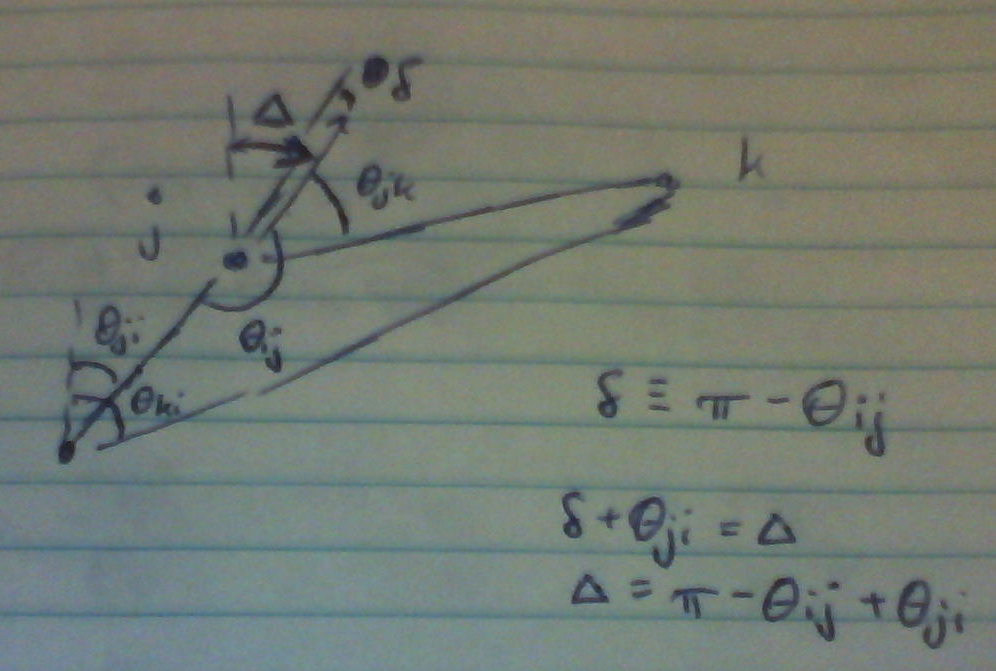
\includegraphics[width=\textwidth]{geometry.png}
\caption{}
\label{fig:geometry}
\end{figure}

\subsection{older stuff}

The basic background describing agent dynamics and the measurement models has been described in the writeup for the case with both bearing and range measurements of landmarks. New work considers the removal of feature range measurements, while retaining knowledge of feature global positions. The estimation task is still to estimate the vehicle's inertial position, velocity, and heading angle. Egocentric feature measurements are treated exactly as before, but there are no range measurements. Similarly, the expectation of the landmark bearing derived from using another agent's measurements is a straightforward function of vehicle state estimates. The computed landmark bearing, which is treated as a measurement, is a nonlinear function of state estimates from both vehicles, interagent measurements, and the other agent's feature bearing measurement.

As previously, consider estimation executed by agent $i$. Agent $j$ makes bearing measurements $\theta_{kj}$ of feature $k$ and shares these measurements and required state estimates and covariances. As previously, the computed value $\theta_{ki}$ for the feature bearing from agent $i$ to feature $k$ is a function of the interagent position vector and the vector from $j$ to $k$:

\begin{equation}
\theta_{ki} = \theta_{ji} + \arctan{\frac{ 2\rho_{ji}\rho_{kj}\sin{(\psi_i - \psi_j + \theta_{ji} - \theta_{kj})} }{ \rho_{ji}^2 + \rho_{ki}^2 - \rho_{kj}^2 } }
\label{eq:thetaki}
\end{equation}

$\rho_{ji}$, $\theta_{ji}$, and $\theta_{kj}$ are measurements; $psi_i$ and $\psi_j$ are estimates from agent $i$ and agent $j$ respectively, as before. Now, $\rho_{kj}$ is a nonlinear function of $j$'s estimated state, rather than a measurement:

\begin{equation}
\hat{\rho}_{kj} = \| [\hat{C}_{b^j/n}]\B{r}_k - \hat{\B{r}}_j \|
\label{eq:rhokj}
\end{equation}

$[\hat{C}_{b^j/n}]$ is the direction cosine matrix from the inertial reference to agent $j$'s body reference frame, and is a function of $\hat{\psi}_j$ only. $\B{r}_k$ is known and $\B{r}_j$ is estimated.

The process for treating the egocentric measurements is entirely standard in the field of sequential state estimation. The treatment of the other agent's measurements proceeds as below:

\begin{enumerate}
\item Compute the expectation of $\theta_{ki}$ from agent $i$'s estimated state.
\item Compute the ``measured'' value of $\theta_{ki}$ from Eqs. \ref{eq:thetaki} and \ref{eq:rhokj}.
\item Compute the covariance associated with the ``measurements'' using the method of statistical linearization employed previously with measured range and bearing. In this case, the output \B{y} is a vector of length $m$, where $m$ is the number of features observed by agent $j$. \B{y} is a nonlinear function of a $6+m$ vector \B{x}, defined as $\B{x} = \begin{bmatrix}
\hat{\psi}_i & \hat{\psi}_j & \tilde{\rho}_{ji} & \tilde{\theta}_{ji} & \hat{r}_{jx} & \hat{r}_{jy} & \theta_{1j} & \theta_{2j} \dots \theta_{mj}
\end{bmatrix}^T$. The covariance matrix $R_x$ associated with \B{x} is formed from the known sensor variances and the covariance matrices of $i$ and $j$. The use of multiple estimated states from agent $j$ means that $R_x$ is not diagonal in general. The description of \B{x}, $R_x$, and Eqs. \ref{eq:thetaki}-\ref{eq:rhokj} are sufficient to compute sigma vectors and approximate the output covariance $R_y$.
\end{enumerate}

\section{Simulation results}

Preliminary simulations are conducted with accelerometer variances of $0.05$, gyroscope variance of $0.01$, and feature bearing variance of $0.01$.. Interagent range and bearing variance varies for comparison. Measurements are shared at the full rate (10 Hz). Tables \ref{tab:sig_ar10}-\ref{tab:sig_ar1} summarize errors. It appears that agent range and bearing variances of $1$ and $.01$ are near the limit at which cooperation is useful, as agent 2 performs similarly in individual and cooperative scenarios with these variances. Agent 1 demonstrates a substantial improvement in accuracy in the cooperative case. When the agent range variance is increased to 10, agent 2's accuracy drops substantially in the cooperative scenario and agent 1 derives no apparently significant benefit. 

Performance drops off very quickly when the agent bearing variance increases. Based on the performance with bearing variance of $.1$ with range variances of $1$ and $.1$, agent range measurements would need to be unreasonably precise to compensate for large agent bearing variances. In the scenario considered, $.01$ is probably near the limit for useful agent bearing variance.

\begin{table}[tb!]
\scriptsize
\centering
\begin{tabular}{c|c|c|c|c|c|c|c|c|c|c|c|}
Case & Agent & $S(\epsilon_{rix})$ & $S(\epsilon_{riy})$ & $S(\epsilon_{u})$ & $S(\epsilon_{v})$ & $S(\epsilon_{\psi})$ & $MSE(r_{ix})$ & $MSE(r_{iy})$ & $MSE(u)$ & $MSE(v)$ & $MSE(\psi)$ \\
Individual & 1& 1.21& 0.761& 0.261& 0.237& 0.0311& 1.63& 0.746& 0.0914& 0.0568& 0.0015 \\
Cooperative & 1& 1.08& 0.774& 0.266& 0.263& 0.0341& 1.52& 0.78& 0.11& 0.0694& 0.00119 \\
Individual & 2& 0.393& 0.275& 0.177& 0.164& 0.0198& 0.449& 0.132& 0.0609& 0.0276& 0.000541 \\
Cooperative & 2& 0.572& 0.435& 0.198& 0.187& 0.038& 0.659& 0.268& 0.0739& 0.0359& 0.00186 \\
\end{tabular}
\caption{Monte Carlo simulations with interagent range variance of 10 and interagent bearing variance of $.01$.}
\label{tab:sig_ar10}
\end{table}

\begin{table}[tb!]
\scriptsize
\centering
\begin{tabular}{c|c|c|c|c|c|c|c|c|c|c|c|}
Case & Agent & $S(\epsilon_{rix})$ & $S(\epsilon_{riy})$ & $S(\epsilon_{u})$ & $S(\epsilon_{v})$ & $S(\epsilon_{\psi})$ & $MSE(r_{ix})$ & $MSE(r_{iy})$ & $MSE(u)$ & $MSE(v)$ & $MSE(\psi)$ \\
Individual & 1& 1.28& 0.776& 0.266& 0.241& 0.0311& 1.81& 0.762& 0.0932& 0.0584& 0.00143 \\
Cooperative & 1& 0.739& 0.631& 0.238& 0.239& 0.0236& 0.743& 0.568& 0.0857& 0.0572& 0.000651 \\
Individual & 2& 0.385& 0.274& 0.179& 0.167& 0.0192& 0.452& 0.13& 0.0613& 0.0287& 0.00052 \\
Cooperative & 2& 0.393& 0.299& 0.172& 0.165& 0.0209& 0.548& 0.139& 0.0668& 0.0293& 0.000629 \\
\end{tabular}
\caption{Monte Carlo simulations with interagent range variance of 1 and interagent bearing variance of $.01$.}
\label{tab:sig_ar1}
\end{table}

\begin{table}[tb!]
\scriptsize
\centering
\begin{tabular}{c|c|c|c|c|c|c|c|c|c|c|c|}
Case & Agent & $S(\epsilon_{rix})$ & $S(\epsilon_{riy})$ & $S(\epsilon_{u})$ & $S(\epsilon_{v})$ & $S(\epsilon_{\psi})$ & $MSE(r_{ix})$ & $MSE(r_{iy})$ & $MSE(u)$ & $MSE(v)$ & $MSE(\psi)$ \\
Individual & 1& 1.14& 0.722& 0.256& 0.237& 0.0309& 1.44& 0.684& 0.0876& 0.0567& 0.00146 \\
Cooperative & 1& 2.22& 1.9& 0.433& 0.352& 0.0631& 5.59& 4.35& 0.268& 0.126& 0.00486 \\
Individual & 2& 0.39& 0.278& 0.175& 0.162& 0.0197& 0.448& 0.138& 0.0613& 0.0268& 0.000558 \\
Cooperative & 2& 0.946& 0.775& 0.282& 0.212& 0.0506& 1.49& 0.775& 0.142& 0.0451& 0.00302 \\
\end{tabular}
\caption{Monte Carlo simulations with interagent range variance of $1$ and interagent bearing variance of $.1$.}
\label{tab:sig_ar1_ab_.1}
\end{table}

\begin{table}[tb!]
\scriptsize
\centering
\begin{tabular}{c|c|c|c|c|c|c|c|c|c|c|c|}
Case & Agent & $S(\epsilon_{rix})$ & $S(\epsilon_{riy})$ & $S(\epsilon_{u})$ & $S(\epsilon_{v})$ & $S(\epsilon_{\psi})$ & $MSE(r_{ix})$ & $MSE(r_{iy})$ & $MSE(u)$ & $MSE(v)$ & $MSE(\psi)$ \\
Individual & 1& 1.28& 0.769& 0.266& 0.237& 0.0316& 1.82& 0.756& 0.0951& 0.057& 0.00149 \\
Cooperative & 1& 1.74& 1.53& 0.369& 0.324& 0.0552& 3.56& 2.91& 0.206& 0.106& 0.00357 \\
Individual & 2& 0.393& 0.283& 0.175& 0.163& 0.0196& 0.47& 0.139& 0.0623& 0.0274& 0.000553 \\
Cooperative & 2& 0.89& 0.718& 0.273& 0.21& 0.048& 1.37& 0.674& 0.135& 0.0448& 0.00275 \\
\end{tabular}
\caption{Monte Carlo simulations with interagent range variance of $.1$ and interagent bearing variance of $.1$.}
\label{tab:sig_ar.1_ab_.1}
\end{table}

\bibliography{../../references}
\bibliographystyle{aiaa}

\end{document}
